% Options for packages loaded elsewhere
\PassOptionsToPackage{unicode}{hyperref}
\PassOptionsToPackage{hyphens}{url}
\PassOptionsToPackage{dvipsnames,svgnames,x11names}{xcolor}
%
\documentclass[
  a4paper,
]{article}

\usepackage{amsmath,amssymb}
\usepackage{iftex}
\ifPDFTeX
  \usepackage[T1]{fontenc}
  \usepackage[utf8]{inputenc}
  \usepackage{textcomp} % provide euro and other symbols
\else % if luatex or xetex
  \usepackage{unicode-math}
  \defaultfontfeatures{Scale=MatchLowercase}
  \defaultfontfeatures[\rmfamily]{Ligatures=TeX,Scale=1}
\fi
\usepackage{lmodern}
\ifPDFTeX\else  
    % xetex/luatex font selection
\fi
% Use upquote if available, for straight quotes in verbatim environments
\IfFileExists{upquote.sty}{\usepackage{upquote}}{}
\IfFileExists{microtype.sty}{% use microtype if available
  \usepackage[]{microtype}
  \UseMicrotypeSet[protrusion]{basicmath} % disable protrusion for tt fonts
}{}
\makeatletter
\@ifundefined{KOMAClassName}{% if non-KOMA class
  \IfFileExists{parskip.sty}{%
    \usepackage{parskip}
  }{% else
    \setlength{\parindent}{0pt}
    \setlength{\parskip}{6pt plus 2pt minus 1pt}}
}{% if KOMA class
  \KOMAoptions{parskip=half}}
\makeatother
\usepackage{xcolor}
\usepackage[top=2.54cm,right=2.54cm,bottom=2.54cm,left=2.54cm]{geometry}
\setlength{\emergencystretch}{3em} % prevent overfull lines
\setcounter{secnumdepth}{-\maxdimen} % remove section numbering
% Make \paragraph and \subparagraph free-standing
\ifx\paragraph\undefined\else
  \let\oldparagraph\paragraph
  \renewcommand{\paragraph}[1]{\oldparagraph{#1}\mbox{}}
\fi
\ifx\subparagraph\undefined\else
  \let\oldsubparagraph\subparagraph
  \renewcommand{\subparagraph}[1]{\oldsubparagraph{#1}\mbox{}}
\fi

\usepackage{color}
\usepackage{fancyvrb}
\newcommand{\VerbBar}{|}
\newcommand{\VERB}{\Verb[commandchars=\\\{\}]}
\DefineVerbatimEnvironment{Highlighting}{Verbatim}{commandchars=\\\{\}}
% Add ',fontsize=\small' for more characters per line
\newenvironment{Shaded}{}{}
\newcommand{\AlertTok}[1]{\textcolor[rgb]{1.00,0.33,0.33}{\textbf{#1}}}
\newcommand{\AnnotationTok}[1]{\textcolor[rgb]{0.42,0.45,0.49}{#1}}
\newcommand{\AttributeTok}[1]{\textcolor[rgb]{0.84,0.23,0.29}{#1}}
\newcommand{\BaseNTok}[1]{\textcolor[rgb]{0.00,0.36,0.77}{#1}}
\newcommand{\BuiltInTok}[1]{\textcolor[rgb]{0.84,0.23,0.29}{#1}}
\newcommand{\CharTok}[1]{\textcolor[rgb]{0.01,0.18,0.38}{#1}}
\newcommand{\CommentTok}[1]{\textcolor[rgb]{0.42,0.45,0.49}{#1}}
\newcommand{\CommentVarTok}[1]{\textcolor[rgb]{0.42,0.45,0.49}{#1}}
\newcommand{\ConstantTok}[1]{\textcolor[rgb]{0.00,0.36,0.77}{#1}}
\newcommand{\ControlFlowTok}[1]{\textcolor[rgb]{0.84,0.23,0.29}{#1}}
\newcommand{\DataTypeTok}[1]{\textcolor[rgb]{0.84,0.23,0.29}{#1}}
\newcommand{\DecValTok}[1]{\textcolor[rgb]{0.00,0.36,0.77}{#1}}
\newcommand{\DocumentationTok}[1]{\textcolor[rgb]{0.42,0.45,0.49}{#1}}
\newcommand{\ErrorTok}[1]{\textcolor[rgb]{1.00,0.33,0.33}{\underline{#1}}}
\newcommand{\ExtensionTok}[1]{\textcolor[rgb]{0.84,0.23,0.29}{\textbf{#1}}}
\newcommand{\FloatTok}[1]{\textcolor[rgb]{0.00,0.36,0.77}{#1}}
\newcommand{\FunctionTok}[1]{\textcolor[rgb]{0.44,0.26,0.76}{#1}}
\newcommand{\ImportTok}[1]{\textcolor[rgb]{0.01,0.18,0.38}{#1}}
\newcommand{\InformationTok}[1]{\textcolor[rgb]{0.42,0.45,0.49}{#1}}
\newcommand{\KeywordTok}[1]{\textcolor[rgb]{0.84,0.23,0.29}{#1}}
\newcommand{\NormalTok}[1]{\textcolor[rgb]{0.14,0.16,0.18}{#1}}
\newcommand{\OperatorTok}[1]{\textcolor[rgb]{0.14,0.16,0.18}{#1}}
\newcommand{\OtherTok}[1]{\textcolor[rgb]{0.44,0.26,0.76}{#1}}
\newcommand{\PreprocessorTok}[1]{\textcolor[rgb]{0.84,0.23,0.29}{#1}}
\newcommand{\RegionMarkerTok}[1]{\textcolor[rgb]{0.42,0.45,0.49}{#1}}
\newcommand{\SpecialCharTok}[1]{\textcolor[rgb]{0.00,0.36,0.77}{#1}}
\newcommand{\SpecialStringTok}[1]{\textcolor[rgb]{0.01,0.18,0.38}{#1}}
\newcommand{\StringTok}[1]{\textcolor[rgb]{0.01,0.18,0.38}{#1}}
\newcommand{\VariableTok}[1]{\textcolor[rgb]{0.89,0.38,0.04}{#1}}
\newcommand{\VerbatimStringTok}[1]{\textcolor[rgb]{0.01,0.18,0.38}{#1}}
\newcommand{\WarningTok}[1]{\textcolor[rgb]{1.00,0.33,0.33}{#1}}

\providecommand{\tightlist}{%
  \setlength{\itemsep}{0pt}\setlength{\parskip}{0pt}}\usepackage{longtable,booktabs,array}
\usepackage{calc} % for calculating minipage widths
% Correct order of tables after \paragraph or \subparagraph
\usepackage{etoolbox}
\makeatletter
\patchcmd\longtable{\par}{\if@noskipsec\mbox{}\fi\par}{}{}
\makeatother
% Allow footnotes in longtable head/foot
\IfFileExists{footnotehyper.sty}{\usepackage{footnotehyper}}{\usepackage{footnote}}
\makesavenoteenv{longtable}
\usepackage{graphicx}
\makeatletter
\def\maxwidth{\ifdim\Gin@nat@width>\linewidth\linewidth\else\Gin@nat@width\fi}
\def\maxheight{\ifdim\Gin@nat@height>\textheight\textheight\else\Gin@nat@height\fi}
\makeatother
% Scale images if necessary, so that they will not overflow the page
% margins by default, and it is still possible to overwrite the defaults
% using explicit options in \includegraphics[width, height, ...]{}
\setkeys{Gin}{width=\maxwidth,height=\maxheight,keepaspectratio}
% Set default figure placement to htbp
\makeatletter
\def\fps@figure{htbp}
\makeatother

\makeatletter
\makeatother
\makeatletter
\makeatother
\makeatletter
\@ifpackageloaded{caption}{}{\usepackage{caption}}
\AtBeginDocument{%
\ifdefined\contentsname
  \renewcommand*\contentsname{Tabla de contenidos}
\else
  \newcommand\contentsname{Tabla de contenidos}
\fi
\ifdefined\listfigurename
  \renewcommand*\listfigurename{Listado de Figuras}
\else
  \newcommand\listfigurename{Listado de Figuras}
\fi
\ifdefined\listtablename
  \renewcommand*\listtablename{Listado de Tablas}
\else
  \newcommand\listtablename{Listado de Tablas}
\fi
\ifdefined\figurename
  \renewcommand*\figurename{Figura}
\else
  \newcommand\figurename{Figura}
\fi
\ifdefined\tablename
  \renewcommand*\tablename{Tabla}
\else
  \newcommand\tablename{Tabla}
\fi
}
\@ifpackageloaded{float}{}{\usepackage{float}}
\floatstyle{ruled}
\@ifundefined{c@chapter}{\newfloat{codelisting}{h}{lop}}{\newfloat{codelisting}{h}{lop}[chapter]}
\floatname{codelisting}{Listado}
\newcommand*\listoflistings{\listof{codelisting}{Listado de Listados}}
\makeatother
\makeatletter
\@ifpackageloaded{caption}{}{\usepackage{caption}}
\@ifpackageloaded{subcaption}{}{\usepackage{subcaption}}
\makeatother
\makeatletter
\@ifpackageloaded{tcolorbox}{}{\usepackage[skins,breakable]{tcolorbox}}
\makeatother
\makeatletter
\@ifundefined{shadecolor}{\definecolor{shadecolor}{rgb}{.97, .97, .97}}
\makeatother
\makeatletter
\makeatother
\makeatletter
\makeatother
\ifLuaTeX
\usepackage[bidi=basic]{babel}
\else
\usepackage[bidi=default]{babel}
\fi
\babelprovide[main,import]{spanish}
% get rid of language-specific shorthands (see #6817):
\let\LanguageShortHands\languageshorthands
\def\languageshorthands#1{}
\ifLuaTeX
  \usepackage{selnolig}  % disable illegal ligatures
\fi
\usepackage[]{biblatex}
\addbibresource{../../../../references.bib}
\IfFileExists{bookmark.sty}{\usepackage{bookmark}}{\usepackage{hyperref}}
\IfFileExists{xurl.sty}{\usepackage{xurl}}{} % add URL line breaks if available
\urlstyle{same} % disable monospaced font for URLs
\hypersetup{
  pdftitle={Visualización de datos en tiempo real con python},
  pdfauthor={Edison Achalma},
  pdflang={es},
  colorlinks=true,
  linkcolor={blue},
  filecolor={Maroon},
  citecolor={Blue},
  urlcolor={Blue},
  pdfcreator={LaTeX via pandoc}}

\title{Visualización de datos en tiempo real con python}
\usepackage{etoolbox}
\makeatletter
\providecommand{\subtitle}[1]{% add subtitle to \maketitle
  \apptocmd{\@title}{\par {\large #1 \par}}{}{}
}
\makeatother
\subtitle{Descubre cómo visualizar y actualizar datos en tiempo real
para tomar decisiones más informadas y ágiles}
\author{Edison Achalma}
\date{2023-07-01}

\begin{document}
\maketitle
\ifdefined\Shaded\renewenvironment{Shaded}{\begin{tcolorbox}[interior hidden, frame hidden, sharp corners, borderline west={3pt}{0pt}{shadecolor}, boxrule=0pt, breakable, enhanced]}{\end{tcolorbox}}\fi

\hypertarget{introducciuxf3n-a-la-visualizaciuxf3n-de-datos-en-tiempo-real}{%
\section{Introducción a la visualización de datos en tiempo
real}\label{introducciuxf3n-a-la-visualizaciuxf3n-de-datos-en-tiempo-real}}

La visualización de datos en tiempo real se refiere a la representación
gráfica de datos que se actualizan constantemente y en tiempo real. Es
una técnica poderosa que permite analizar y comprender la información en
tiempo real, lo que resulta fundamental en entornos donde la velocidad
del cambio es crítica.

Imagina tener acceso a datos en tiempo real de una red de sensores, un
sistema de monitoreo o incluso redes sociales. La capacidad de
visualizar y comprender rápidamente estos datos te brinda una ventaja
competitiva al tomar decisiones más informadas y ágiles.

\hypertarget{quuxe9-es-la-visualizaciuxf3n-de-datos-en-tiempo-real-y-por-quuxe9-es-importante}{%
\subsection{Qué es la visualización de datos en tiempo real y por qué es
importante}\label{quuxe9-es-la-visualizaciuxf3n-de-datos-en-tiempo-real-y-por-quuxe9-es-importante}}

La visualización de datos en tiempo real implica mostrar información
actualizada a medida que los datos se generan o se modifican. A
diferencia de la visualización estática, donde los datos son estáticos y
no cambian, la visualización de datos en tiempo real te permite seguir
el ritmo de los eventos en tiempo real.

Esta técnica es especialmente útil en situaciones donde la toma de
decisiones rápidas es fundamental. Por ejemplo, en el ámbito financiero,
la visualización de datos en tiempo real permite monitorear los cambios
en los precios de las acciones o en los indicadores económicos al
instante, lo que facilita la identificación de oportunidades o riesgos.

En resumen, la visualización de datos en tiempo real te ayuda a estar al
tanto de la velocidad del cambio, tomar decisiones más inteligentes y
estratégicas, y adaptarte rápidamente a las condiciones cambiantes del
entorno.

\hypertarget{casos-de-uso-de-la-visualizaciuxf3n-de-datos-en-tiempo-real}{%
\subsection{Casos de uso de la visualización de datos en tiempo
real}\label{casos-de-uso-de-la-visualizaciuxf3n-de-datos-en-tiempo-real}}

La visualización de datos en tiempo real encuentra aplicaciones en
diversos campos. Algunos casos de uso comunes incluyen:

\begin{itemize}
\item
  Monitoreo de sistemas y redes: permite visualizar el rendimiento, la
  disponibilidad y los eventos en tiempo real de sistemas informáticos,
  redes de comunicación y otros sistemas complejos.
\item
  Análisis de datos financieros: proporciona una visión en tiempo real
  de los cambios en los precios de acciones, divisas, materias primas y
  otros activos financieros.
\item
  Seguimiento de redes sociales: permite visualizar y analizar en tiempo
  real los datos generados en las redes sociales, como menciones de
  marca, tendencias y sentimiento del público.
\item
  Monitoreo de sensores y dispositivos IoT: facilita la visualización de
  datos generados por sensores en tiempo real, como temperatura,
  humedad, presión, etc.
\end{itemize}

Estos son solo algunos ejemplos, pero la visualización de datos en
tiempo real es una técnica versátil que se puede aplicar en una amplia
gama de escenarios para mejorar la comprensión y la toma de decisiones.

\hypertarget{introducciuxf3n-a-las-bibliotecas-y-herramientas-utilizadas-en-la-visualizaciuxf3n-de-datos-en-tiempo-real}{%
\subsection{Introducción a las bibliotecas y herramientas utilizadas en
la visualización de datos en tiempo
real}\label{introducciuxf3n-a-las-bibliotecas-y-herramientas-utilizadas-en-la-visualizaciuxf3n-de-datos-en-tiempo-real}}

En la visualización de datos en tiempo real, existen varias bibliotecas
y herramientas populares que facilitan la creación de gráficos y
visualizaciones interactivas. Algunas de las principales bibliotecas
utilizadas en Python son:

\begin{itemize}
\item
  Matplotlib: una biblioteca ampliamente utilizada que ofrece una gran
  flexibilidad para crear visualizaciones estáticas y animadas.
\item
  Plotly: una biblioteca de visualización interactiva que permite crear
  gráficos interactivos y actualizables en tiempo real.
\item
  Bokeh: otra biblioteca de visualización interactiva que se enfoca en
  la creación de visualizaciones interactivas basadas en la web.
\end{itemize}

Estas bibliotecas proporcionan una amplia gama de opciones para crear
gráficos en tiempo real, desde gráficos de líneas y gráficos de barras
hasta mapas de calor y gráficos de dispersión interactivos.

\hypertarget{gruxe1ficos-en-streaming}{%
\section{Gráficos en streaming}\label{gruxe1ficos-en-streaming}}

Los gráficos en streaming son una forma efectiva de visualizar datos que
se actualizan constantemente en tiempo real. Te permiten observar la
evolución de los datos a medida que se generan o se modifican, lo que
resulta especialmente útil cuando necesitas monitorear tendencias o
cambios en tiempo real.

\hypertarget{cuxf3mo-visualizar-datos-que-se-actualizan-constantemente-en-tiempo-real}{%
\subsection{Cómo visualizar datos que se actualizan constantemente en
tiempo
real}\label{cuxf3mo-visualizar-datos-que-se-actualizan-constantemente-en-tiempo-real}}

La visualización de datos en tiempo real requiere una estrategia para
capturar y procesar los datos en tiempo real, así como una forma de
representarlos gráficamente. Para visualizar datos que se actualizan
constantemente, puedes seguir estos pasos:

\begin{enumerate}
\def\labelenumi{\arabic{enumi}.}
\item
  Obtener los datos: primero, debes establecer una fuente de datos en
  tiempo real, como un flujo de datos de sensores, una API de terceros o
  una base de datos en continuo crecimiento. Es importante contar con un
  mecanismo para recibir los datos a medida que se generan o se
  actualizan.
\item
  Procesar los datos: una vez que recibes los datos, es necesario
  procesarlos y estructurarlos adecuadamente para su visualización. Esto
  puede implicar filtrar, transformar o agregar los datos según tus
  necesidades.
\item
  Actualizar la visualización: una vez que tienes los datos preparados,
  debes actualizar la visualización en tiempo real. Esto implica
  refrescar el gráfico con los nuevos datos a medida que llegan.
  Dependiendo de la biblioteca que estés utilizando, puede haber métodos
  específicos para actualizar los gráficos en streaming.
\end{enumerate}

\hypertarget{utilizaciuxf3n-de-bibliotecas-como-matplotlib-plotly-y-bokeh-para-crear-gruxe1ficos-en-streaming}{%
\subsection{Utilización de bibliotecas como Matplotlib, Plotly y Bokeh
para crear gráficos en
streaming}\label{utilizaciuxf3n-de-bibliotecas-como-matplotlib-plotly-y-bokeh-para-crear-gruxe1ficos-en-streaming}}

Las bibliotecas de visualización como Matplotlib, Plotly y Bokeh ofrecen
herramientas y funcionalidades para crear gráficos en streaming en
Python. Estas bibliotecas te permiten representar los datos en tiempo
real de forma interactiva y dinámica.

\begin{enumerate}
\def\labelenumi{\arabic{enumi}.}
\item
  Matplotlib: Matplotlib proporciona funcionalidades para crear gráficos
  en streaming mediante el uso de la función \texttt{FuncAnimation}.
  Puedes actualizar los datos del gráfico en tiempo real a través de un
  bucle y llamar a la función \texttt{FuncAnimation} para refrescar la
  visualización.
\item
  Plotly: Plotly es una biblioteca que se destaca en la creación de
  gráficos interactivos en tiempo real. Puedes utilizar la función
  \texttt{update\_traces} para actualizar los datos en un gráfico
  existente. También ofrece la posibilidad de crear visualizaciones en
  streaming utilizando la función \texttt{stream}.
\item
  Bokeh: Bokeh permite crear gráficos interactivos en streaming mediante
  su modelo de actualización de datos. Puedes utilizar la función
  \texttt{ColumnDataSource} para almacenar los datos y actualizarlos en
  tiempo real. Luego, puedes enlazar los datos actualizados al gráfico y
  visualizarlos en streaming.
\end{enumerate}

\hypertarget{uso-de-bibliotecas-para-datos-en-continuo}{%
\subsection{Uso de bibliotecas para datos en
continuo}\label{uso-de-bibliotecas-para-datos-en-continuo}}

Una de las bibliotecas más utilizadas para visualización en tiempo real
es Matplotlib. Aunque Matplotlib es conocida principalmente por crear
gráficos estáticos, también podemos aprovechar sus capacidades para
visualizar datos en tiempo real. Podemos utilizar la función
\texttt{plt.plot()} en un bucle mientras los datos se actualizan
continuamente para lograr la visualización en tiempo real.

\begin{Shaded}
\begin{Highlighting}[]
\ImportTok{import}\NormalTok{ seaborn }\ImportTok{as}\NormalTok{ sns}
\ImportTok{import}\NormalTok{ geopandas }\ImportTok{as}\NormalTok{ gpd}
\ImportTok{from}\NormalTok{ bokeh.models }\ImportTok{import}\NormalTok{ ColumnDataSource}
\ImportTok{from}\NormalTok{ bokeh.plotting }\ImportTok{import}\NormalTok{ figure, curdoc}
\ImportTok{import}\NormalTok{ matplotlib.pyplot }\ImportTok{as}\NormalTok{ plt}
\ImportTok{import}\NormalTok{ numpy }\ImportTok{as}\NormalTok{ np}

\CommentTok{\# Configuración inicial}
\NormalTok{fig, ax }\OperatorTok{=}\NormalTok{ plt.subplots()}
\NormalTok{x }\OperatorTok{=}\NormalTok{ np.linspace(}\DecValTok{0}\NormalTok{, }\DecValTok{10}\NormalTok{, }\DecValTok{100}\NormalTok{)}
\NormalTok{y }\OperatorTok{=}\NormalTok{ np.sin(x)}

\CommentTok{\# Actualización en tiempo real}
\ControlFlowTok{for}\NormalTok{ i }\KeywordTok{in} \BuiltInTok{range}\NormalTok{(}\DecValTok{100}\NormalTok{):}
\NormalTok{    y }\OperatorTok{=}\NormalTok{ np.sin(x }\OperatorTok{+}\NormalTok{ i }\OperatorTok{*} \FloatTok{0.1}\NormalTok{)}
\NormalTok{    ax.clear()}
\NormalTok{    ax.plot(x, y)}
\NormalTok{    plt.pause(}\FloatTok{0.1}\NormalTok{)}

\NormalTok{plt.show()}
\end{Highlighting}
\end{Shaded}

\begin{figure}[H]

{\centering 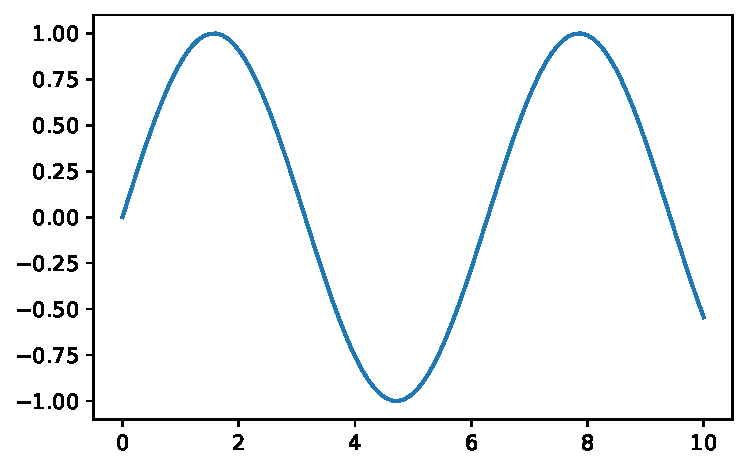
\includegraphics{index_files/figure-pdf/cell-2-output-1.pdf}

}

\end{figure}

En el código anterior, utilizamos Matplotlib para crear un gráfico de
línea en tiempo real. En cada iteración del bucle, actualizamos los
datos y redibujamos el gráfico utilizando \texttt{ax.clear()} para
eliminar el contenido anterior y \texttt{ax.plot()} para trazar los
nuevos datos. Luego, utilizamos \texttt{plt.pause()} para pausar
brevemente la ejecución y permitir la actualización visual.

Otra biblioteca popular para visualización en tiempo real es Bokeh.
Bokeh nos permite crear gráficos interactivos y actualizables en un
navegador web. Con su funcionalidad de streaming de datos, podemos
conectar nuestros datos en continuo y observar cómo evolucionan en
tiempo real.

\begin{Shaded}
\begin{Highlighting}[]
\CommentTok{\# Configuración inicial}
\NormalTok{p }\OperatorTok{=}\NormalTok{ figure()}
\NormalTok{x }\OperatorTok{=}\NormalTok{ np.linspace(}\DecValTok{0}\NormalTok{, }\DecValTok{10}\NormalTok{, }\DecValTok{100}\NormalTok{)}
\NormalTok{y }\OperatorTok{=}\NormalTok{ np.sin(x)}

\CommentTok{\# Actualización en tiempo real}
\NormalTok{source }\OperatorTok{=}\NormalTok{ ColumnDataSource(data}\OperatorTok{=}\BuiltInTok{dict}\NormalTok{(x}\OperatorTok{=}\NormalTok{x, y}\OperatorTok{=}\NormalTok{y))}
\NormalTok{p.line(x}\OperatorTok{=}\StringTok{\textquotesingle{}x\textquotesingle{}}\NormalTok{, y}\OperatorTok{=}\StringTok{\textquotesingle{}y\textquotesingle{}}\NormalTok{, source}\OperatorTok{=}\NormalTok{source)}


\KeywordTok{def}\NormalTok{ update():}
\NormalTok{    new\_y }\OperatorTok{=}\NormalTok{ np.sin(x }\OperatorTok{+}\NormalTok{ curdoc().count }\OperatorTok{*} \FloatTok{0.1}\NormalTok{)}
\NormalTok{    source.data }\OperatorTok{=} \BuiltInTok{dict}\NormalTok{(x}\OperatorTok{=}\NormalTok{x, y}\OperatorTok{=}\NormalTok{new\_y)}
\NormalTok{    curdoc().count }\OperatorTok{+=} \DecValTok{1}


\NormalTok{curdoc().count }\OperatorTok{=} \DecValTok{0}
\NormalTok{curdoc().add\_periodic\_callback(update, }\DecValTok{100}\NormalTok{)}

\NormalTok{curdoc().title }\OperatorTok{=} \StringTok{"Visualización en tiempo real"}
\NormalTok{curdoc().add\_root(p)}
\end{Highlighting}
\end{Shaded}

En este ejemplo de Bokeh, utilizamos la función \texttt{figure()} para
crear un nuevo gráfico y \texttt{p.line()} para trazar la línea inicial.
Luego, definimos una función \texttt{update()} que actualiza los datos y
los asigna a la fuente de datos \texttt{ColumnDataSource}. Utilizamos
\texttt{curdoc().add\_periodic\_callback()} para llamar a la función
\texttt{update()} periódicamente y actualizar los datos en tiempo real.

\hypertarget{ejemplos-pruxe1cticos-de-gruxe1ficos-de-luxedneas-y-gruxe1ficos-de-barras-en-streaming}{%
\subsection{Ejemplos prácticos de gráficos de líneas y gráficos de
barras en
streaming}\label{ejemplos-pruxe1cticos-de-gruxe1ficos-de-luxedneas-y-gruxe1ficos-de-barras-en-streaming}}

Veamos algunos ejemplos prácticos de cómo crear gráficos de líneas y
gráficos de barras en streaming utilizando las bibliotecas mencionadas:

\hypertarget{gruxe1fico-de-luxedneas-en-streaming-con-matplotlib}{%
\subsubsection{Gráfico de líneas en streaming con
Matplotlib}\label{gruxe1fico-de-luxedneas-en-streaming-con-matplotlib}}

\begin{Shaded}
\begin{Highlighting}[]
\ImportTok{import}\NormalTok{ matplotlib.pyplot }\ImportTok{as}\NormalTok{ plt}
\ImportTok{import}\NormalTok{ numpy }\ImportTok{as}\NormalTok{ np}
\ImportTok{from}\NormalTok{ matplotlib.animation }\ImportTok{import}\NormalTok{ FuncAnimation}

\CommentTok{\# Crear una figura y un eje}
\NormalTok{fig, ax }\OperatorTok{=}\NormalTok{ plt.subplots()}

\CommentTok{\# Inicializar los datos}
\NormalTok{x }\OperatorTok{=}\NormalTok{ np.linspace(}\DecValTok{0}\NormalTok{, }\DecValTok{10}\NormalTok{, }\DecValTok{100}\NormalTok{)}
\NormalTok{y }\OperatorTok{=}\NormalTok{ np.sin(x)}

\CommentTok{\# Crear la línea inicial}
\NormalTok{line, }\OperatorTok{=}\NormalTok{ ax.plot(x, y)}

\CommentTok{\# Función de actualización en tiempo real}
\KeywordTok{def}\NormalTok{ update(i):}
    \CommentTok{\# Generar nuevos datos}
\NormalTok{    y\_new }\OperatorTok{=}\NormalTok{ np.sin(x }\OperatorTok{+}\NormalTok{ i}\OperatorTok{/}\DecValTok{10}\NormalTok{)}

    \CommentTok{\# Actualizar los datos de la línea}
\NormalTok{    line.set\_ydata(y\_new)}

    \CommentTok{\# Ajustar el rango de los ejes si es necesario}
\NormalTok{    ax.relim()}
\NormalTok{    ax.autoscale\_view()}

    \CommentTok{\# Devolver la línea actualizada}
    \ControlFlowTok{return}\NormalTok{ line,}

\CommentTok{\# Crear la animación en tiempo real}
\NormalTok{ani }\OperatorTok{=}\NormalTok{ FuncAnimation(fig, update, frames}\OperatorTok{=}\DecValTok{100}\NormalTok{, interval}\OperatorTok{=}\DecValTok{200}\NormalTok{)}

\CommentTok{\# Mostrar el gráfico en streaming}
\NormalTok{plt.show()}
\end{Highlighting}
\end{Shaded}

\begin{figure}[H]

{\centering 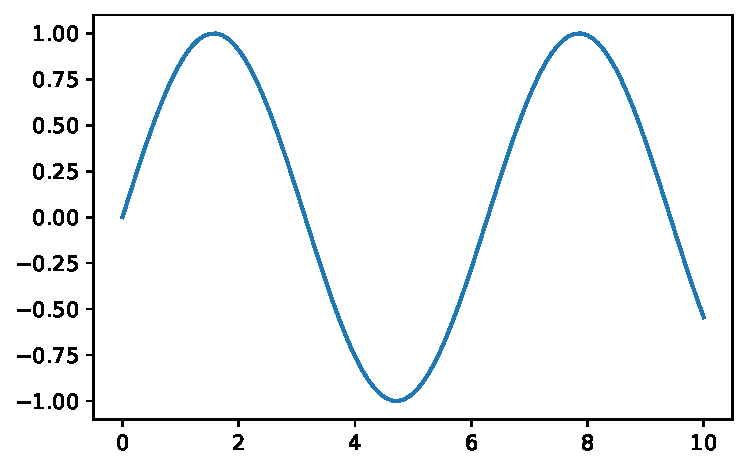
\includegraphics{index_files/figure-pdf/cell-4-output-1.pdf}

}

\end{figure}

En Matplotlib, podemos lograr la actualización de gráficos en tiempo
real utilizando la función \texttt{plt.pause()} dentro de un bucle.
Veamos un ejemplo:

\begin{Shaded}
\begin{Highlighting}[]
\CommentTok{\# Configuración inicial}
\NormalTok{fig, ax }\OperatorTok{=}\NormalTok{ plt.subplots()}
\NormalTok{x }\OperatorTok{=}\NormalTok{ np.linspace(}\DecValTok{0}\NormalTok{, }\DecValTok{10}\NormalTok{, }\DecValTok{100}\NormalTok{)}
\NormalTok{y }\OperatorTok{=}\NormalTok{ np.sin(x)}

\CommentTok{\# Actualización en tiempo real}
\ControlFlowTok{for}\NormalTok{ i }\KeywordTok{in} \BuiltInTok{range}\NormalTok{(}\DecValTok{100}\NormalTok{):}
\NormalTok{    y }\OperatorTok{=}\NormalTok{ np.sin(x }\OperatorTok{+}\NormalTok{ i }\OperatorTok{*} \FloatTok{0.1}\NormalTok{)}
\NormalTok{    ax.clear()}
\NormalTok{    ax.plot(x, y)}
\NormalTok{    plt.pause(}\FloatTok{0.1}\NormalTok{)}

\NormalTok{plt.show()}
\end{Highlighting}
\end{Shaded}

\begin{figure}[H]

{\centering 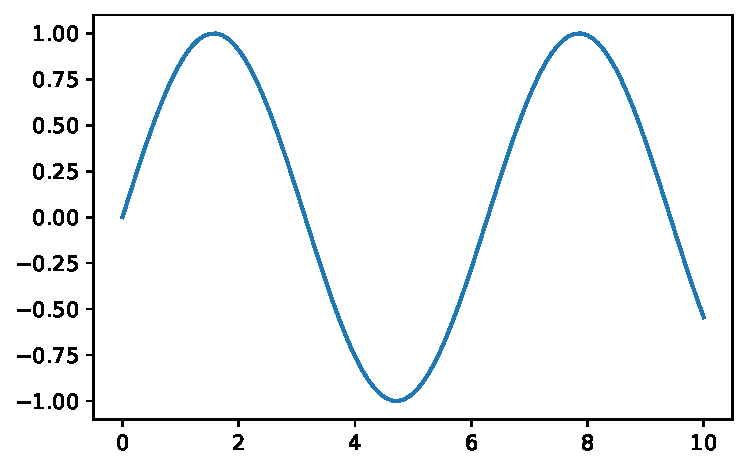
\includegraphics{index_files/figure-pdf/cell-5-output-1.pdf}

}

\end{figure}

En este ejemplo, creamos un gráfico de línea que se actualiza en tiempo
real. En cada iteración del bucle, generamos nuevos datos y los trazamos
utilizando \texttt{ax.plot()}. Utilizamos \texttt{ax.clear()} para
eliminar el contenido anterior y \texttt{plt.pause()} para pausar
brevemente la ejecución y permitir la actualización visual.

\hypertarget{gruxe1fico-de-barras-en-streaming-con-plotly}{%
\subsubsection{Gráfico de barras en streaming con
Plotly}\label{gruxe1fico-de-barras-en-streaming-con-plotly}}

\begin{Shaded}
\begin{Highlighting}[]
\ImportTok{import}\NormalTok{ plotly.graph\_objects }\ImportTok{as}\NormalTok{ go}
\ImportTok{import}\NormalTok{ numpy }\ImportTok{as}\NormalTok{ np}

\CommentTok{\# Crear los datos iniciales}
\NormalTok{x }\OperatorTok{=}\NormalTok{ np.arange(}\DecValTok{10}\NormalTok{)}
\NormalTok{y }\OperatorTok{=}\NormalTok{ np.random.rand(}\DecValTok{10}\NormalTok{)}

\CommentTok{\# Crear la figura y las barras iniciales}
\NormalTok{fig }\OperatorTok{=}\NormalTok{ go.Figure(data}\OperatorTok{=}\NormalTok{[go.Bar(x}\OperatorTok{=}\NormalTok{x, y}\OperatorTok{=}\NormalTok{y)])}

\CommentTok{\# Actualizar las barras en tiempo real}
\KeywordTok{def}\NormalTok{ update():}
    \ControlFlowTok{while} \VariableTok{True}\NormalTok{:}
        \CommentTok{\# Generar nuevos datos}
\NormalTok{        y\_new }\OperatorTok{=}\NormalTok{ np.random.rand(}\DecValTok{10}\NormalTok{)}

        \CommentTok{\# Actualizar las barras}
\NormalTok{        fig.data[}\DecValTok{0}\NormalTok{].y }\OperatorTok{=}\NormalTok{ y\_new}

        \CommentTok{\# Actualizar el layout si es necesario}
\NormalTok{        fig.update\_layout(autosize}\OperatorTok{=}\VariableTok{False}\NormalTok{, width}\OperatorTok{=}\DecValTok{500}\NormalTok{, height}\OperatorTok{=}\DecValTok{400}\NormalTok{)}

        \CommentTok{\# Renderizar el gráfico en tiempo real}
\NormalTok{        fig.show()}

\CommentTok{\# Iniciar la actualización en tiempo real}
\NormalTok{update()}
\end{Highlighting}
\end{Shaded}

Estos ejemplos te brindan una idea de cómo crear gráficos en streaming
con Matplotlib y Plotly.

\hypertarget{gruxe1ficos-interactivos-actualizados-automuxe1ticamente}{%
\section{Gráficos interactivos actualizados
automáticamente}\label{gruxe1ficos-interactivos-actualizados-automuxe1ticamente}}

Los gráficos interactivos actualizados automáticamente son una forma
poderosa de visualizar datos en tiempo real. Estos gráficos se
actualizan automáticamente a medida que llegan nuevos datos, lo que te
permite monitorear y analizar la evolución de los datos en tiempo real
de manera interactiva.

\hypertarget{cuxf3mo-crear-gruxe1ficos-que-se-actualicen-automuxe1ticamente-a-medida-que-llegan-nuevos-datos}{%
\subsection{Cómo crear gráficos que se actualicen automáticamente a
medida que llegan nuevos
datos}\label{cuxf3mo-crear-gruxe1ficos-que-se-actualicen-automuxe1ticamente-a-medida-que-llegan-nuevos-datos}}

Para crear gráficos que se actualicen automáticamente a medida que
llegan nuevos datos, puedes seguir estos pasos:

\begin{enumerate}
\def\labelenumi{\arabic{enumi}.}
\item
  Establecer una fuente de datos en tiempo real: debes tener una fuente
  de datos en tiempo real que proporcione los nuevos datos a medida que
  se generan o se actualizan. Esto puede ser un flujo de datos en
  continuo, una API en tiempo real o una base de datos que se actualiza
  constantemente.
\item
  Configurar la visualización inicial: antes de que lleguen los nuevos
  datos, configura la visualización inicial del gráfico. Puedes
  establecer el tipo de gráfico, los ejes, los colores y cualquier otro
  elemento visual que desees mostrar.
\item
  Preparar la estructura de datos: para recibir y almacenar los nuevos
  datos, debes preparar una estructura adecuada. Puede ser una lista, un
  array o una estructura de datos más compleja dependiendo de las
  necesidades de tu aplicación.
\item
  Actualizar los datos y la visualización: a medida que llegan los
  nuevos datos, debes agregarlos a la estructura de datos existente.
  Luego, actualiza la visualización del gráfico con los nuevos datos.
  Esto puede implicar la actualización de las series de datos, la
  adición de nuevos puntos en un gráfico de dispersión o el ajuste de
  las áreas en un gráfico de áreas.
\item
  Actualizar automáticamente la visualización: para lograr que la
  visualización se actualice automáticamente, debes utilizar las
  funcionalidades de las bibliotecas de visualización adecuadas, como
  Plotly y Bokeh. Estas bibliotecas ofrecen métodos específicos para
  actualizar los gráficos en tiempo real, como \texttt{update\_traces}
  en Plotly y \texttt{stream} en Bokeh.
\end{enumerate}

\hypertarget{utilizaciuxf3n-de-bibliotecas-como-plotly-y-bokeh-para-crear-gruxe1ficos-interactivos-actualizados-en-tiempo-real}{%
\subsection{Utilización de bibliotecas como Plotly y Bokeh para crear
gráficos interactivos actualizados en tiempo
real}\label{utilizaciuxf3n-de-bibliotecas-como-plotly-y-bokeh-para-crear-gruxe1ficos-interactivos-actualizados-en-tiempo-real}}

Las bibliotecas Plotly y Bokeh son excelentes opciones para crear
gráficos interactivos actualizados en tiempo real en Python.

\begin{enumerate}
\def\labelenumi{\arabic{enumi}.}
\item
  Plotly: Plotly es una biblioteca de visualización que proporciona una
  amplia gama de tipos de gráficos interactivos y dinámicos. Ofrece
  funcionalidades específicas para la visualización en tiempo real, como
  \texttt{update\_traces}, que te permite actualizar los datos de las
  trazas en un gráfico existente. También puedes utilizar la función
  \texttt{stream} para recibir datos en tiempo real y agregarlos al
  gráfico en streaming.
\item
  Bokeh: Bokeh es otra biblioteca de visualización que se centra en la
  creación de gráficos interactivos y dinámicos. Ofrece funcionalidades
  para la visualización en tiempo real, como \texttt{ColumnDataSource},
  que te permite enlazar los datos actualizados al gráfico y
  actualizarlo automáticamente. También puedes utilizar la función
  \texttt{stream} para recibir datos en tiempo real y agregarlos al
  gráfico.
\end{enumerate}

\hypertarget{ejemplos-pruxe1cticos-de-gruxe1ficos-de-dispersiuxf3n-y-gruxe1ficos-de-uxe1reas-actualizados-en-tiempo-real}{%
\subsection{Ejemplos prácticos de gráficos de dispersión y gráficos de
áreas actualizados en tiempo
real}\label{ejemplos-pruxe1cticos-de-gruxe1ficos-de-dispersiuxf3n-y-gruxe1ficos-de-uxe1reas-actualizados-en-tiempo-real}}

A continuación, te presento ejemplos prácticos de cómo crear gráficos de
dispersión y gráficos de áreas actualizados en tiempo real utilizando
las bibliotecas Plotly y Bokeh:

\hypertarget{gruxe1fico-de-dispersiuxf3n-actualizado-en-tiempo-real-con-plotly}{%
\subsubsection{Gráfico de dispersión actualizado en tiempo real con
Plotly}\label{gruxe1fico-de-dispersiuxf3n-actualizado-en-tiempo-real-con-plotly}}

\begin{Shaded}
\begin{Highlighting}[]
\ImportTok{import}\NormalTok{ plotly.graph\_objects }\ImportTok{as}\NormalTok{ go}
\ImportTok{import}\NormalTok{ random}

\CommentTok{\# Crear una figura y un conjunto de datos iniciales}
\NormalTok{fig }\OperatorTok{=}\NormalTok{ go.Figure(data}\OperatorTok{=}\NormalTok{go.Scatter(x}\OperatorTok{=}\NormalTok{[], y}\OperatorTok{=}\NormalTok{[], mode}\OperatorTok{=}\StringTok{"markers"}\NormalTok{))}

\CommentTok{\# Configurar el diseño del gráfico}
\NormalTok{fig.update\_layout(}
\NormalTok{    title}\OperatorTok{=}\StringTok{"Gráfico de dispersión en tiempo real"}\NormalTok{,}
\NormalTok{    xaxis\_title}\OperatorTok{=}\StringTok{"Eje X"}\NormalTok{,}
\NormalTok{    yaxis\_title}\OperatorTok{=}\StringTok{"Eje Y"}
\NormalTok{)}

\CommentTok{\# Función para actualizar el gráfico en tiempo real}
\KeywordTok{def}\NormalTok{ update\_scatter():}
    \CommentTok{\# Generar nuevos datos}
\NormalTok{    x }\OperatorTok{=}\NormalTok{ random.randint(}\DecValTok{0}\NormalTok{, }\DecValTok{10}\NormalTok{)}
\NormalTok{    y }\OperatorTok{=}\NormalTok{ random.randint(}\DecValTok{0}\NormalTok{, }\DecValTok{10}\NormalTok{)}

    \CommentTok{\# Actualizar los datos del gráfico}
\NormalTok{    fig.add\_trace(go.Scatter(x}\OperatorTok{=}\NormalTok{[x], y}\OperatorTok{=}\NormalTok{[y], mode}\OperatorTok{=}\StringTok{"markers"}\NormalTok{))}

    \CommentTok{\# Actualizar el gráfico}
\NormalTok{    fig.show()}

\CommentTok{\# Actualizar el gráfico cada segundo}
\ControlFlowTok{while} \VariableTok{True}\NormalTok{:}
\NormalTok{    update\_scatter()}
\end{Highlighting}
\end{Shaded}

\hypertarget{gruxe1fico-de-uxe1reas-actualizado-en-tiempo-real-con-bokeh}{%
\subsubsection{Gráfico de áreas actualizado en tiempo real con
Bokeh}\label{gruxe1fico-de-uxe1reas-actualizado-en-tiempo-real-con-bokeh}}

\begin{Shaded}
\begin{Highlighting}[]
\ImportTok{from}\NormalTok{ bokeh.plotting }\ImportTok{import}\NormalTok{ figure, curdoc}
\ImportTok{from}\NormalTok{ random }\ImportTok{import}\NormalTok{ randint}
\ImportTok{from}\NormalTok{ bokeh.models }\ImportTok{import}\NormalTok{ ColumnDataSource}
\ImportTok{from}\NormalTok{ bokeh.layouts }\ImportTok{import}\NormalTok{ column}

\CommentTok{\# Crear una figura y un origen de datos}
\NormalTok{p }\OperatorTok{=}\NormalTok{ figure(title}\OperatorTok{=}\StringTok{"Gráfico de áreas en tiempo real"}\NormalTok{, x\_axis\_label}\OperatorTok{=}\StringTok{"Eje X"}\NormalTok{, y\_axis\_label}\OperatorTok{=}\StringTok{"Eje Y"}\NormalTok{)}
\NormalTok{source }\OperatorTok{=}\NormalTok{ ColumnDataSource(data}\OperatorTok{=}\BuiltInTok{dict}\NormalTok{(x}\OperatorTok{=}\NormalTok{[], y}\OperatorTok{=}\NormalTok{[]))}

\CommentTok{\# Configurar el gráfico de áreas}
\NormalTok{p.patch(x}\OperatorTok{=}\StringTok{"x"}\NormalTok{, y}\OperatorTok{=}\StringTok{"y"}\NormalTok{, source}\OperatorTok{=}\NormalTok{source, alpha}\OperatorTok{=}\FloatTok{0.4}\NormalTok{, line\_width}\OperatorTok{=}\DecValTok{2}\NormalTok{)}

\CommentTok{\# Función para actualizar el gráfico en tiempo real}
\KeywordTok{def}\NormalTok{ update\_area():}
    \CommentTok{\# Generar nuevos datos}
\NormalTok{    x }\OperatorTok{=}\NormalTok{ randint(}\DecValTok{0}\NormalTok{, }\DecValTok{10}\NormalTok{)}
\NormalTok{    y }\OperatorTok{=}\NormalTok{ randint(}\DecValTok{0}\NormalTok{, }\DecValTok{10}\NormalTok{)}

    \CommentTok{\# Actualizar los datos del origen de datos}
\NormalTok{    source.stream(}\BuiltInTok{dict}\NormalTok{(x}\OperatorTok{=}\NormalTok{[x], y}\OperatorTok{=}\NormalTok{[y]))}

\CommentTok{\# Configurar el documento Bokeh}
\NormalTok{curdoc().add\_root(column(p))}

\CommentTok{\# Actualizar el gráfico cada segundo}
\NormalTok{curdoc().add\_periodic\_callback(update\_area, }\DecValTok{1000}\NormalTok{)}
\end{Highlighting}
\end{Shaded}

En Bokeh, podemos utilizar la función \texttt{ColumnDataSource} y el
método \texttt{stream()} para lograr la actualización en tiempo real.
Veamos un ejemplo:

\begin{Shaded}
\begin{Highlighting}[]
\CommentTok{\# Configuración inicial}
\NormalTok{p }\OperatorTok{=}\NormalTok{ figure()}
\NormalTok{x }\OperatorTok{=}\NormalTok{ np.linspace(}\DecValTok{0}\NormalTok{, }\DecValTok{10}\NormalTok{, }\DecValTok{100}\NormalTok{)}
\NormalTok{y }\OperatorTok{=}\NormalTok{ np.sin(x)}

\CommentTok{\# Actualización en tiempo real}
\NormalTok{source }\OperatorTok{=}\NormalTok{ ColumnDataSource(data}\OperatorTok{=}\BuiltInTok{dict}\NormalTok{(x}\OperatorTok{=}\NormalTok{x, y}\OperatorTok{=}\NormalTok{y))}
\NormalTok{p.line(x}\OperatorTok{=}\StringTok{\textquotesingle{}x\textquotesingle{}}\NormalTok{, y}\OperatorTok{=}\StringTok{\textquotesingle{}y\textquotesingle{}}\NormalTok{, source}\OperatorTok{=}\NormalTok{source)}


\KeywordTok{def}\NormalTok{ update():}
\NormalTok{    new\_y }\OperatorTok{=}\NormalTok{ np.sin(x }\OperatorTok{+}\NormalTok{ curdoc().count }\OperatorTok{*} \FloatTok{0.1}\NormalTok{)}
\NormalTok{    source.stream(}\BuiltInTok{dict}\NormalTok{(x}\OperatorTok{=}\NormalTok{x, y}\OperatorTok{=}\NormalTok{new\_y), rollover}\OperatorTok{=}\DecValTok{100}\NormalTok{)}


\NormalTok{curdoc().count }\OperatorTok{=} \DecValTok{0}
\NormalTok{curdoc().add\_periodic\_callback(update, }\DecValTok{100}\NormalTok{)}

\NormalTok{curdoc().title }\OperatorTok{=} \StringTok{"Actualización en tiempo real"}
\NormalTok{curdoc().add\_root(p)}
\end{Highlighting}
\end{Shaded}

En este ejemplo de Bokeh, utilizamos la función
\texttt{ColumnDataSource} para almacenar nuestros datos y el método
\texttt{stream()} para actualizarlos en tiempo real. La función
\texttt{update()} genera nuevos datos y los agrega a la fuente de datos
utilizando \texttt{source.stream()}. Utilizamos
\texttt{curdoc().add\_periodic\_callback()} para llamar a la función
\texttt{update()} periódicamente y actualizar los datos en tiempo real.

\hypertarget{visualizaciuxf3n-de-datos-en-tiempo-real-en-aplicaciones-web}{%
\section{Visualización de datos en tiempo real en aplicaciones
web}\label{visualizaciuxf3n-de-datos-en-tiempo-real-en-aplicaciones-web}}

La visualización de datos en tiempo real también se puede integrar en
aplicaciones web, lo que permite mostrar gráficos actualizados
automáticamente y en tiempo real directamente en un navegador web. Esto
brinda una experiencia interactiva a los usuarios y les permite obtener
información en tiempo real de manera conveniente.

\hypertarget{integraciuxf3n-de-gruxe1ficos-en-tiempo-real-en-aplicaciones-web-utilizando-bibliotecas-como-flask-y-dash}{%
\subsection{Integración de gráficos en tiempo real en aplicaciones web
utilizando bibliotecas como Flask y
Dash}\label{integraciuxf3n-de-gruxe1ficos-en-tiempo-real-en-aplicaciones-web-utilizando-bibliotecas-como-flask-y-dash}}

Existen varias bibliotecas de Python que facilitan la integración de
gráficos en tiempo real en aplicaciones web. Algunas de las bibliotecas
más populares son Flask y Dash.

\begin{itemize}
\item
  Flask: Flask es un framework web ligero y flexible que permite
  construir aplicaciones web de manera sencilla. Puedes utilizar Flask
  para crear un servidor web y enviar los datos actualizados desde el
  servidor al navegador. Con la ayuda de bibliotecas de visualización
  como Plotly o Bokeh, puedes generar gráficos en tiempo real y
  enviarlos al navegador para su visualización.
\item
  Dash: Dash es un framework de Python diseñado específicamente para la
  construcción de aplicaciones web interactivas. Dash combina la
  facilidad de uso de Flask con las capacidades de visualización de
  Plotly. Puedes utilizar Dash para crear una aplicación web en la que
  los gráficos se actualicen automáticamente a medida que llegan nuevos
  datos.
\end{itemize}

\hypertarget{ejemplos-pruxe1cticos-de-visualizaciuxf3n-de-datos-en-tiempo-real-en-aplicaciones-web-interactivas}{%
\subsection{Ejemplos prácticos de visualización de datos en tiempo real
en aplicaciones web
interactivas}\label{ejemplos-pruxe1cticos-de-visualizaciuxf3n-de-datos-en-tiempo-real-en-aplicaciones-web-interactivas}}

A continuación, te presento un ejemplo práctico utilizando Dash para
crear una aplicación web interactiva con gráficos en tiempo real:

\begin{Shaded}
\begin{Highlighting}[]
\ImportTok{import}\NormalTok{ dash}
\ImportTok{import}\NormalTok{ dash\_core\_components }\ImportTok{as}\NormalTok{ dcc}
\ImportTok{import}\NormalTok{ dash\_html\_components }\ImportTok{as}\NormalTok{ html}
\ImportTok{from}\NormalTok{ dash.dependencies }\ImportTok{import}\NormalTok{ Input, Output}
\ImportTok{import}\NormalTok{ plotly.graph\_objs }\ImportTok{as}\NormalTok{ go}
\ImportTok{import}\NormalTok{ random}
\ImportTok{import}\NormalTok{ time}

\CommentTok{\# Crear la aplicación Dash}
\NormalTok{app }\OperatorTok{=}\NormalTok{ dash.Dash(}\VariableTok{\_\_name\_\_}\NormalTok{)}

\CommentTok{\# Definir el diseño de la aplicación}
\NormalTok{app.layout }\OperatorTok{=}\NormalTok{ html.Div([}
\NormalTok{    html.H1(}\StringTok{"Visualización de datos en tiempo real"}\NormalTok{),}
\NormalTok{    dcc.Graph(}\BuiltInTok{id}\OperatorTok{=}\StringTok{"real{-}time{-}graph"}\NormalTok{),}
\NormalTok{    dcc.Interval(}\BuiltInTok{id}\OperatorTok{=}\StringTok{"interval{-}component"}\NormalTok{, interval}\OperatorTok{=}\DecValTok{1000}\NormalTok{, n\_intervals}\OperatorTok{=}\DecValTok{0}\NormalTok{)}
\NormalTok{])}

\CommentTok{\# Callback para actualizar el gráfico en tiempo real}
\AttributeTok{@app.callback}\NormalTok{(Output(}\StringTok{"real{-}time{-}graph"}\NormalTok{, }\StringTok{"figure"}\NormalTok{),}
\NormalTok{              [Input(}\StringTok{"interval{-}component"}\NormalTok{, }\StringTok{"n\_intervals"}\NormalTok{)])}
\KeywordTok{def}\NormalTok{ update\_real\_time\_graph(n):}
    \CommentTok{\# Generar nuevos datos}
\NormalTok{    x }\OperatorTok{=} \BuiltInTok{list}\NormalTok{(}\BuiltInTok{range}\NormalTok{(}\DecValTok{10}\NormalTok{))}
\NormalTok{    y }\OperatorTok{=}\NormalTok{ [random.randint(}\DecValTok{0}\NormalTok{, }\DecValTok{100}\NormalTok{) }\ControlFlowTok{for}\NormalTok{ \_ }\KeywordTok{in} \BuiltInTok{range}\NormalTok{(}\DecValTok{10}\NormalTok{)]}

    \CommentTok{\# Crear la figura del gráfico}
\NormalTok{    figure }\OperatorTok{=}\NormalTok{ go.Figure(data}\OperatorTok{=}\NormalTok{[go.Scatter(x}\OperatorTok{=}\NormalTok{x, y}\OperatorTok{=}\NormalTok{y, mode}\OperatorTok{=}\StringTok{"lines"}\NormalTok{)])}

    \CommentTok{\# Configurar el diseño del gráfico}
\NormalTok{    figure.update\_layout(}
\NormalTok{        title}\OperatorTok{=}\StringTok{"Gráfico en tiempo real"}\NormalTok{,}
\NormalTok{        xaxis\_title}\OperatorTok{=}\StringTok{"Tiempo"}\NormalTok{,}
\NormalTok{        yaxis\_title}\OperatorTok{=}\StringTok{"Valor"}
\NormalTok{    )}

    \CommentTok{\# Retornar la figura del gráfico}
    \ControlFlowTok{return}\NormalTok{ figure}

\CommentTok{\# Ejecutar la aplicación}
\ControlFlowTok{if} \VariableTok{\_\_name\_\_} \OperatorTok{==} \StringTok{"\_\_main\_\_"}\NormalTok{:}
\NormalTok{    app.run\_server(debug}\OperatorTok{=}\VariableTok{True}\NormalTok{)}
\end{Highlighting}
\end{Shaded}

En este ejemplo, se utiliza Dash para crear una aplicación web con un
gráfico en tiempo real. El gráfico se actualiza automáticamente cada
segundo con nuevos datos generados aleatoriamente. Puedes personalizar
este ejemplo para adaptarlo a tus propios datos y necesidades.

\hypertarget{visualizaciuxf3n-de-datos-geoespaciales}{%
\section{Visualización de datos
geoespaciales}\label{visualizaciuxf3n-de-datos-geoespaciales}}

\hypertarget{utilizaciuxf3n-de-datos-geoespaciales}{%
\subsection{Utilización de datos
geoespaciales}\label{utilizaciuxf3n-de-datos-geoespaciales}}

La visualización de datos geoespaciales nos permite representar
información en relación con su ubicación geográfica. Esto resulta
especialmente útil cuando queremos explorar patrones, tendencias y
relaciones en datos que tienen una dimensión espacial.

Para utilizar datos geoespaciales en nuestras visualizaciones,
necesitamos fuentes de datos que contengan información geográfica, como
coordenadas de latitud y longitud, códigos postales o nombres de
ciudades. Estos datos pueden provenir de diversas fuentes, como bases de
datos especializadas, servicios de mapas en línea o conjuntos de datos
abiertos.

Una de las bibliotecas más populares para trabajar con datos
geoespaciales en Python es GeoPandas. GeoPandas es una extensión de la
biblioteca Pandas que agrega capacidades espaciales, lo que nos permite
manipular y visualizar datos geoespaciales de manera sencilla.

Veamos un ejemplo básico de cómo utilizar GeoPandas para visualizar
datos geoespaciales en un mapa:

\begin{Shaded}
\begin{Highlighting}[]
\CommentTok{\# pip install geopandas}

\CommentTok{\# Cargar datos geoespaciales}
\NormalTok{world }\OperatorTok{=}\NormalTok{ gpd.read\_file(gpd.datasets.get\_path(}\StringTok{\textquotesingle{}naturalearth\_lowres\textquotesingle{}}\NormalTok{))}

\CommentTok{\# Visualizar mapa}
\NormalTok{world.plot()}

\CommentTok{\# Mostrar el mapa}
\NormalTok{plt.show()}
\end{Highlighting}
\end{Shaded}

\begin{figure}[H]

{\centering 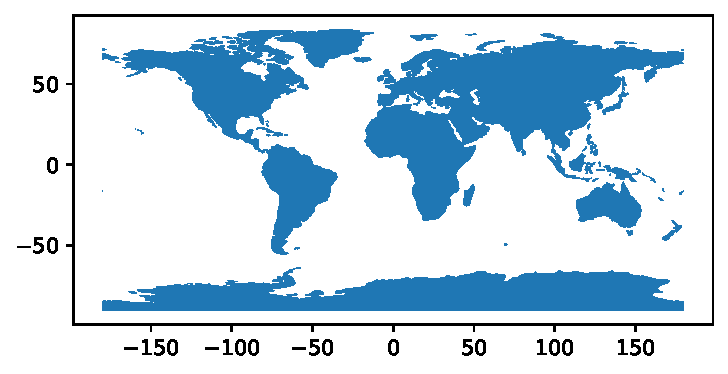
\includegraphics{index_files/figure-pdf/cell-7-output-1.pdf}

}

\end{figure}

En este ejemplo, cargamos un conjunto de datos geoespaciales que
contiene información sobre los países del mundo. Utilizamos el método
\texttt{plot()} para visualizar los datos en un mapa. Luego, utilizamos
\texttt{plt.show()} para mostrar el mapa en una ventana emergente.

Además de GeoPandas, existen otras bibliotecas como Folium y Plotly que
también nos permiten crear visualizaciones interactivas de datos
geoespaciales. Estas bibliotecas nos brindan opciones avanzadas para
personalizar los mapas, agregar capas adicionales y explorar datos de
manera interactiva.

La visualización de datos geoespaciales nos ayuda a comprender mejor la
distribución geográfica de los datos y revelar patrones ocultos que
podrían pasar desapercibidos en otro tipo de gráficos. Explorar y
visualizar datos en un contexto geoespacial agrega un nivel adicional de
información y nos permite tomar decisiones basadas en la ubicación.

\hypertarget{mapas-de-calor-y-mapas-temuxe1ticos}{%
\subsection{Mapas de calor y mapas
temáticos}\label{mapas-de-calor-y-mapas-temuxe1ticos}}

Los mapas de calor y los mapas temáticos son poderosas herramientas de
visualización que nos permiten representar datos geoespaciales de manera
más significativa. Estos mapas nos ayudan a identificar patrones y
tendencias en función de valores numéricos o categorías específicas.

Un mapa de calor utiliza colores para representar la intensidad o
densidad de un fenómeno en un área geográfica. Es ideal para mostrar la
concentración de datos o la variación espacial de una variable, como la
temperatura, la densidad de población o el rendimiento de un producto en
diferentes regiones.

Por otro lado, los mapas temáticos se utilizan para representar
categorías o clases específicas en un mapa. Cada categoría se asocia con
un color o un patrón único, lo que permite visualizar la distribución
espacial de diferentes características o atributos, como el tipo de
vegetación, la diversidad cultural o las tasas de criminalidad en
diferentes áreas.

Para crear mapas de calor y mapas temáticos, podemos utilizar
bibliotecas especializadas como Matplotlib, Seaborn y GeoPandas. Estas
bibliotecas nos brindan una variedad de funciones y herramientas para
personalizar la apariencia de nuestros mapas y resaltar la información
más relevante.

Aquí tienes un ejemplo básico de cómo crear un mapa de calor utilizando
Seaborn:

\begin{Shaded}
\begin{Highlighting}[]
\CommentTok{\# pip install seaborn matplotlib}

\CommentTok{\# Cargar datos}
\NormalTok{data }\OperatorTok{=}\NormalTok{ np.random.rand(}\DecValTok{10}\NormalTok{, }\DecValTok{10}\NormalTok{)}

\CommentTok{\# Crear mapa de calor}
\NormalTok{sns.heatmap(data)}

\CommentTok{\# Mostrar el mapa de calor}
\NormalTok{plt.show()}
\end{Highlighting}
\end{Shaded}

\begin{figure}[H]

{\centering 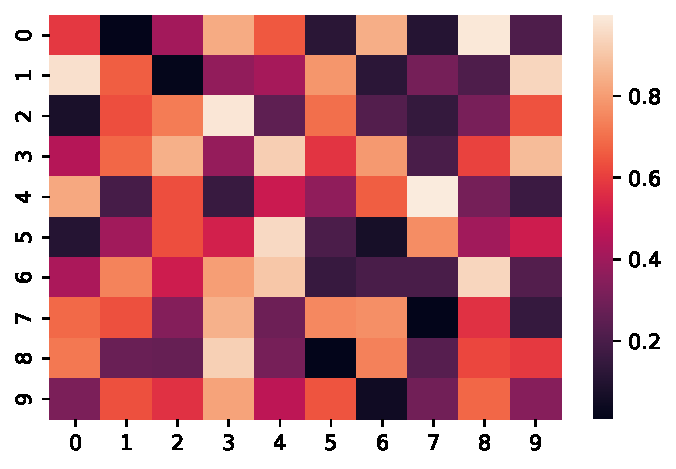
\includegraphics{index_files/figure-pdf/cell-8-output-1.pdf}

}

\end{figure}

En este ejemplo, cargamos nuestros datos y utilizamos la función
\texttt{heatmap()} de Seaborn para crear el mapa de calor. Luego,
utilizamos \texttt{plt.show()} para mostrar el mapa en una ventana
emergente.

Recuerda que la elección de colores es importante en los mapas de calor
y mapas temáticos. Debes seleccionar una paleta de colores que sea
perceptualmente equilibrada y que permita una fácil interpretación de
los datos.

Explorar datos geoespaciales a través de mapas de calor y mapas
temáticos nos brinda una visión más completa y comprensible de los
patrones y relaciones espaciales. Estas visualizaciones nos ayudan a
tomar decisiones más informadas y a comunicar eficazmente la información
a otras personas.

\hypertarget{casos-de-estudio-y-ejemplos-pruxe1cticos}{%
\section{Casos de estudio y ejemplos
prácticos}\label{casos-de-estudio-y-ejemplos-pruxe1cticos}}

La visualización de datos en tiempo real tiene aplicaciones en una
amplia variedad de dominios y escenarios. A continuación, exploraremos
algunos casos de estudio y ejemplos prácticos de cómo se puede aplicar
esta técnica en diferentes áreas:

\hypertarget{aplicaciuxf3n-de-la-visualizaciuxf3n-de-datos-en-tiempo-real-en-diferentes-dominios}{%
\subsection{Aplicación de la visualización de datos en tiempo real en
diferentes
dominios}\label{aplicaciuxf3n-de-la-visualizaciuxf3n-de-datos-en-tiempo-real-en-diferentes-dominios}}

Finanzas: En el campo de las finanzas, la visualización de datos en
tiempo real es fundamental para el monitoreo de los mercados, la
detección de patrones y tendencias, y la toma de decisiones ágiles. Los
gráficos en tiempo real permiten a los analistas y traders visualizar la
evolución de los precios de las acciones, divisas y otros instrumentos
financieros, así como la detección de anomalías y eventos importantes.

Monitoreo de sistemas: En entornos tecnológicos y de infraestructura, la
visualización de datos en tiempo real es esencial para el monitoreo y la
gestión de sistemas y redes. Los gráficos en tiempo real permiten
visualizar métricas clave, como la carga del servidor, el tráfico de
red, la disponibilidad de recursos y otros indicadores de rendimiento.
Esto ayuda a identificar problemas, optimizar la capacidad y tomar
acciones correctivas de manera rápida.

Redes sociales: Las redes sociales generan grandes cantidades de datos
en tiempo real. La visualización de estos datos en tiempo real permite
comprender la dinámica de la participación de los usuarios, la
propagación de contenido y las tendencias emergentes. Los gráficos en
tiempo real pueden mostrar la actividad de los usuarios, los
comentarios, las interacciones y las menciones relacionadas con temas
específicos, lo que proporciona información valiosa para campañas de
marketing, análisis de sentimiento y toma de decisiones estratégicas.

\hypertarget{ejemplos-de-visualizaciuxf3n-de-datos-en-tiempo-real-en-escenarios-reales}{%
\subsection{Ejemplos de visualización de datos en tiempo real en
escenarios
reales}\label{ejemplos-de-visualizaciuxf3n-de-datos-en-tiempo-real-en-escenarios-reales}}

A continuación, presentaremos algunos ejemplos prácticos de
visualización de datos en tiempo real en escenarios reales:

\begin{itemize}
\item
  Monitoreo de tráfico en tiempo real: Mediante el uso de sensores y
  cámaras, es posible recopilar datos sobre el tráfico vehicular en
  tiempo real. Estos datos pueden visualizarse en mapas interactivos y
  gráficos en tiempo real para proporcionar información sobre el flujo
  de tráfico, los patrones de congestión y las rutas más eficientes.
\item
  Seguimiento de redes sociales: Las empresas pueden utilizar
  herramientas de visualización en tiempo real para monitorear las redes
  sociales y obtener información sobre la opinión de los usuarios, las
  tendencias emergentes y las campañas de marketing. Esto permite
  adaptar rápidamente las estrategias y tomar decisiones informadas
  basadas en los datos en tiempo real.
\item
  Monitoreo de sistemas de energía: En la industria energética, la
  visualización de datos en tiempo real es esencial para monitorear y
  gestionar los sistemas de generación y distribución de energía. Los
  gráficos en tiempo real pueden mostrar datos como la demanda de
  energía, la producción, los precios y otros factores relevantes para
  optimizar la eficiencia y la calidad del suministro de energía.
\end{itemize}

\hypertarget{consideraciones-de-rendimiento-y-escalabilidad}{%
\section{Consideraciones de rendimiento y
escalabilidad}\label{consideraciones-de-rendimiento-y-escalabilidad}}

Cuando trabajamos con grandes volúmenes de datos en tiempo real, es
importante tener en cuenta varios factores para garantizar un
rendimiento óptimo y una escalabilidad adecuada en la visualización de
datos. A continuación, exploraremos algunas consideraciones y
estrategias clave:

\hypertarget{factores-a-tener-en-cuenta-al-trabajar-con-grandes-voluxfamenes-de-datos-en-tiempo-real}{%
\subsection{Factores a tener en cuenta al trabajar con grandes volúmenes
de datos en tiempo
real}\label{factores-a-tener-en-cuenta-al-trabajar-con-grandes-voluxfamenes-de-datos-en-tiempo-real}}

\begin{enumerate}
\def\labelenumi{\arabic{enumi}.}
\item
  \textbf{Velocidad de procesamiento}: Los datos en tiempo real se
  generan y actualizan rápidamente, por lo que es fundamental contar con
  una infraestructura que permita procesarlos a alta velocidad. Esto
  implica utilizar técnicas de procesamiento paralelo, optimización de
  consultas y sistemas distribuidos para manejar la carga de trabajo.
\item
  \textbf{Latencia}: La latencia es el tiempo transcurrido entre la
  generación de los datos y su visualización. Para garantizar una
  experiencia en tiempo real, es esencial minimizar la latencia. Esto
  implica utilizar sistemas de transmisión de datos eficientes,
  minimizar las operaciones de lectura/escritura y optimizar el
  rendimiento de las consultas.
\item
  \textbf{Escalabilidad}: A medida que aumenta el volumen de datos y la
  cantidad de usuarios que acceden a la visualización en tiempo real, es
  necesario que el sistema sea escalable. Esto implica utilizar
  arquitecturas distribuidas, sistemas de procesamiento en paralelo y
  técnicas de particionamiento de datos para garantizar que el sistema
  pueda manejar la carga sin degradar el rendimiento.
\item
  \textbf{Optimización de consultas}: Para garantizar un rendimiento
  eficiente, es importante optimizar las consultas de datos. Esto
  implica utilizar índices adecuados, estructuras de datos optimizadas y
  técnicas de filtrado y agregación para reducir el tiempo de respuesta
  y minimizar el procesamiento innecesario.
\end{enumerate}

\hypertarget{estrategias-para-optimizar-el-rendimiento-y-la-escalabilidad-de-la-visualizaciuxf3n-de-datos-en-tiempo-real}{%
\subsection{Estrategias para optimizar el rendimiento y la escalabilidad
de la visualización de datos en tiempo
real}\label{estrategias-para-optimizar-el-rendimiento-y-la-escalabilidad-de-la-visualizaciuxf3n-de-datos-en-tiempo-real}}

\begin{enumerate}
\def\labelenumi{\arabic{enumi}.}
\item
  \textbf{Caché de datos}: Utilizar técnicas de caché puede mejorar
  significativamente el rendimiento al reducir la necesidad de acceder a
  la fuente de datos en cada consulta. Almacenar en caché los resultados
  de consultas anteriores y mantenerlos actualizados puede acelerar la
  generación de visualizaciones en tiempo real.
\item
  \textbf{Procesamiento en tiempo real}: En lugar de procesar todos los
  datos en tiempo real, es posible aplicar técnicas de procesamiento en
  tiempo real para filtrar, resumir o agregar los datos antes de
  visualizarlos. Esto permite reducir la carga de trabajo en el momento
  de la visualización y mejorar el rendimiento general del sistema.
\item
  \textbf{Distribución de carga}: Distribuir la carga de trabajo en
  varios nodos o servidores puede mejorar la escalabilidad del sistema.
  Esto implica utilizar técnicas de particionamiento de datos, balanceo
  de carga y paralelismo para distribuir eficientemente el procesamiento
  de datos entre diferentes recursos.
\item
  \textbf{Compresión de datos}: La compresión de datos puede reducir el
  espacio de almacenamiento y el ancho de banda necesario para
  transmitir los datos. Utilizar algoritmos de compresión adecuados
  puede mejorar la eficiencia del sistema y reducir los costos asociados
  con el almacenamiento y la transmisión de datos.
\end{enumerate}

\hypertarget{conclusiones-y-recursos-adicionales}{%
\section{Conclusiones y recursos
adicionales}\label{conclusiones-y-recursos-adicionales}}

En conclusión, la visualización de datos en tiempo real es una poderosa
herramienta que nos permite tomar decisiones informadas y ágiles en
entornos dinámicos. Al utilizar bibliotecas y herramientas como
Matplotlib, Plotly, Bokeh, Flask y Dash, podemos crear visualizaciones
interactivas y actualizadas automáticamente que nos permiten explorar y
comprender los datos en tiempo real.

Algunos conceptos clave y mejores prácticas a tener en cuenta son:

\begin{itemize}
\tightlist
\item
  Comprender el dominio y los requisitos específicos del problema antes
  de diseñar visualizaciones en tiempo real.
\item
  Utilizar bibliotecas adecuadas como Matplotlib, Plotly y Bokeh para
  crear gráficos en streaming e interactivos.
\item
  Considerar la escalabilidad y el rendimiento al trabajar con grandes
  volúmenes de datos en tiempo real.
\item
  Implementar estrategias de optimización como el caché de datos, el
  procesamiento en tiempo real y la distribución de carga.
\item
  Mantenerse actualizado con los avances en las bibliotecas y
  herramientas de visualización de datos en tiempo real.
\end{itemize}

Recursos adicionales para aprender más sobre la visualización de datos
en tiempo real con Python:

\begin{itemize}
\tightlist
\item
  \href{https://matplotlib.org/stable/contents.html}{Documentación
  oficial de Matplotlib}
\item
  \href{https://plotly.com/python/}{Documentación oficial de Plotly}
\item
  \href{https://docs.bokeh.org/en/latest/index.html}{Documentación
  oficial de Bokeh}
\item
  \href{https://flask.palletsprojects.com/}{Documentación oficial de
  Flask}
\item
  \href{https://dash.plotly.com/}{Documentación oficial de Dash}
\end{itemize}

Estos recursos proporcionan información detallada, ejemplos prácticos y
tutoriales que te ayudarán a explorar y dominar la visualización de
datos en tiempo real con Python.

\hypertarget{publicaciones-similares}{%
\section{Publicaciones Similares}\label{publicaciones-similares}}

Si te interesó este artículo, te recomendamos que explores otros blogs y
recursos relacionados que pueden ampliar tus conocimientos. Aquí te dejo
algunas sugerencias:

\begin{enumerate}
\def\labelenumi{\arabic{enumi}.}
\item
  \href{../2023-06-22-01-introduccion-a-python/index.qmd}{Introducción}
\item
  \href{../2023-06-23-02-variables-expresiones-y-statements-con-python/index.qmd}{Variables,
  expresiones y statements}
\item
  \href{../2023-06-24-03-objetos-de-python/index.qmd}{Objetos de Python}
\item
  \href{../2023-06-25-04-ejecucion-condicional-con-python/index.qmd}{Ejecución
  condicional}
\item
  \href{../2023-06-26-05-iteraciones-con-python/index.qmd}{Iteraciones}
\item
  \href{../2023-06-27-06-funciones-con-python/index.qmd}{Funciones}
\item
  \href{../2023-06-28-07-dataframes-con-python/index.qmd}{Dataframes}
\item
  \href{../2023-06-29-introduccion-a-la-visualizacion-de-datos-con-python/index.qmd}{Introducción
  a la visualización de datos}
\item
  \href{../2023-06-30-graficos-avanzados-con-python/index.qmd}{Gráficos
  avanzados}
\item
  \href{../2023-07-01-visualizacion-de-datos-en-tiempo-real-con-python/index.qmd}{Visualización
  de datos en tiempo real}
\item
  \href{../2023-07-02-visualizacion-de-datos-en-finanzas-con-python/index.qmd}{Visualización
  de datos en finanzas}
\item
  \href{../2023-07-03-visualizacion-de-datos-en-microeconomia-con-python/index.qmd}{Visualización
  de datos en microeconomía}
\item
  \href{../2023-07-04-visualizacion-de-datos-en-macroeconomia-con-python/index.qmd}{Visualización
  de datos en macroeconomía}
\item
  \href{../2023-07-05-visualizacion-de-datos-en-estadistica-con-python/index.qmd}{Visualización
  de datos en estadística}
\item
  \href{../2023-07-06-visualizacion-de-datos-en-econometria-con-python/index.qmd}{Visualización
  de datos en econometría}
\item
  \href{../2023-07-07-mejores-practicas-y-consejos-de-visualizacion-de-datos-con-python/index.qmd}{Mejores
  prácticas y consejos de visualización de datos}
\item
  \href{../2023-07-08-08-prediccion-y-metrica-de-performance-con-python/index.qmd}{Predicción
  y métrica de performance}
\item
  \href{../2023-07-09-09-metodos-de-machine-learning-para-clasificacion-con-python/index.qmd}{Métodos
  de machine learning para clasificación}
\item
  \href{../2023-07-10-10-metodos-de-machine-learning-para-regresion-con-python/index.qmd}{Métodos
  de machine learning para regresión}
\item
  \href{../2023-07-11-11-validacion-cruzada-y-composicion-del-modelo-con-python/index.qmd}{Validación
  cruzada y composición del modelo}
\end{enumerate}

Esperamos que encuentres estas publicaciones igualmente interesantes y
útiles. ¡Disfruta de la lectura!


\printbibliography


\end{document}
